\section{Downfall}
Moghimi\cite{downfall} introduces the first microarchitectural data sampling exploiting the \verb|gather| instruction, named \textit{Gather Data Sampling}. GDS steal the data leaked by the SIMD register buffer, which is the buffer used for vector instructions like AVX-series.
Also, due to the simultaneous multithreading, known as Hyperthreading technology, aggravates the vulnerabilities. The attacker
thread shared the same resources with the victim.

\subsection{Gather Data Sampling}
The \verb|gather| instruction enables user to collect discontinuous data that shares the same base address.
It was initially intended for the vector operation, by collecting the scalar data to form a vector. Then \verb|gather| will
place them in a vector register. However, some of slot is not intended to be filled. Hence, \verb|gather| requires a mask register
offering the mask bits. These bits indicates that, with 1 the data will fill into the corresponding position in vector register, while 0 means the
data is discarded and what's already in register remains untouched.

\begin{figure}[!htbp]
    \centering
    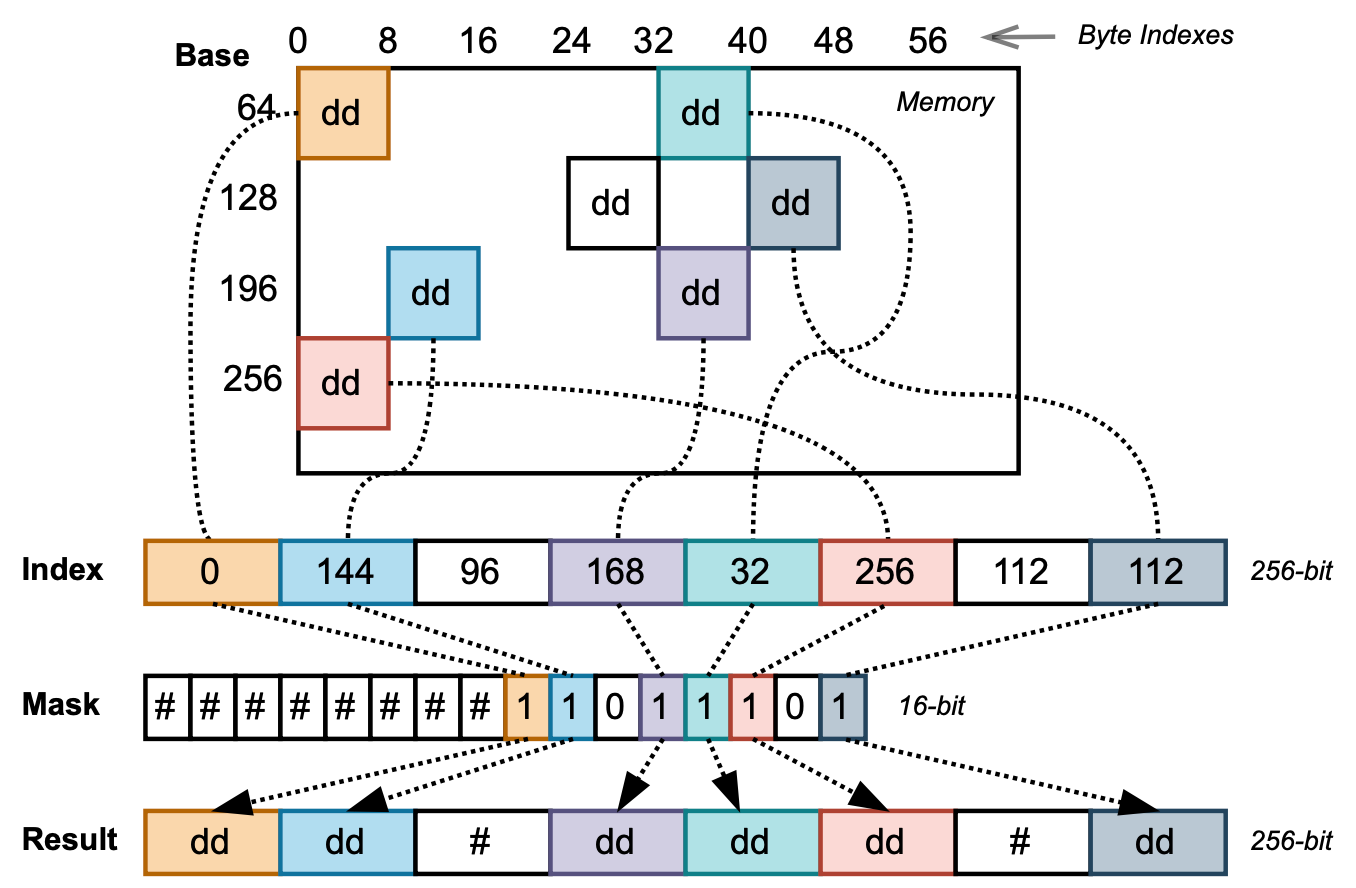
\includegraphics[width=0.99\linewidth]{Figure/gather.png}
    \caption{Execution of gather instruction}
\end{figure}

The author verifies that the processor will
\begin{itemize}
    \item eliminate unnecessary memory reads for unset mask bits, which must be discarded anyway.
    \item reuse the data from the same cache line.
    \item fetch the data in parallel and speculatively and discard results when at least one of the reads has failed.
    \item preserve the intermediate execution state when interrupt comes, and resume.
\end{itemize}

These leads to a critical vulnerability. While the original microarchitectural data sampling has a strict assumption, \verb|gather| eliminates it
by flooding the SIMD register buffer to reserve the possibly sensitive data in the buffer. After that insurance, attacker can easily
perform the MDS attack and steal data from buffer.

\subsection{RISC-V Vector Extension}
Similar to Intel's AVX extension, RISC-V announced its own vector extension leveraging the SIMD technology. Single Instruction Multiple Data (SIMD) 
enables the CPU with parallel processing ability, and utilize the computational resource in backend. Meanwhile, the explicit vector length eliminates
the cost in branching. RISC-V offer additional 32 vector registers and 7 vector CSR for vector operation. But different from x86, the vector registers are the same width with other registers. RISC-V specifies several instruction and state registers (CSR) to group and control them dynamically. For example, \verb|vlen| sets the vector length and \verb|vtype| can groups the vector registers to form a wider vector register. RVV also provides with
rich vector load and store instruction to deal with flexible situation, such as strided and indexed (similar to \verb|gather|).

\begin{figure}[!htbp]
    \centering
    \includesvg[width=0.99\columnwidth]{Figure/xs-arch-kunminghu.svg}
    \caption{The Kunminghu (3rd) architecture of XiangShan}
\end{figure}

The XiangShan will decode instruction to $\mu$ops, which shares similar design with present modern processors, whether it's CISC or RISC. In XiangShan's design, after setting the vector CSR, the vector's decoder will knows how to proceed. The core will decoded the vector computational instruction to several $\mu$ops and reassemble them in commmit stage. But in the execution stage, all $\mu$ops will be executed speculatively and out-of-order, same with the scalar instruction. Meanwhile, there's a speculative execution when the computational instruction is following the control instruction (\verb|vtype|), which is often the case. In this situation, the computation will guess the \verb|vtype| since it always comes from immediate number.

Therefore, the vector instruction and other instruction is treated equally at the execution stage -- they're all $\mu$ops. Scalar instruction and vector 
are executed by the same components, so how can we tell the difference? The answer is we don't, and this enables us to exploit the vector instruction. Similar to Downfall, we can flood the buffers with vector instructions.

\subsection{Exploiting RVV Instruction}
Spotting similar instruction on XiangShan and on Intel, we can make a reasonable guess that the Downfall attack can be replicating on RISC-V.
From Figure 9, the vector buffer is unavailble since vector and scalar has the same execution backend. 

However, the shared resource between scalar and vector, such as the store commit buffer and load buffer, magnifies the attack surface, since
Downfall is restricted to steal data from SIMD register buffers.

\begin{listing}[!htbp]
\begin{minted}{asm}
fence.i
// increase the transient window
vsetvli t0, %[vl], e64, m1 
// Set vector length and element width to 64 bits
vmv.v.x v0, %[mask]
// Move mask to vector register v0
vle32.v v2, (%[indices])
// Load indices into vector register v2
vluxei64.v v1, (%[src]), v2, v0.t
// Load 64-bit elements using indices and mask
vse64.v v1, (%[dst]) Store loaded elements to dst

encode_secret
flush_and_reload
\end{minted}
\label{listing:spectre_vulnerable}
\caption{Downfall with RVV}
\end{listing}

In RVV version of Downfall, we firstly increase the transient window and executes a following instruction required to set vector. Next, we perform
the GDS and encoded the secret to cache line and finally fetch the secret by a traditional flush and reload.

Our alternative guess on exploiting RVV instruction was to leak inaccessible data by setting the mask bits to 0 and bringing it to cache.
By our initial analysis of XiangShan's source code, the guess is possible since the vector load and store instruction will be decoded into 
several $\mu$ops that is similar to regular load and store instruction. But the result will be discarded after checking the mask bits and before commit.
However, this remains to be tested.